\documentclass[a4paper,10pt]{article}

%\usepackage[utf8]{inputenc} 
%\usepackage[square,sort,comma,numbers]{natbib}
%\usepackage[backend=biber,autocite=inline,style=authoryear]{biblatex}
\usepackage[backend=biber,autocite=inline]{biblatex}
\addbibresource{mybib.bib}
\usepackage{a4wide}
\usepackage{amsmath}
\usepackage{amssymb}
\usepackage{amsthm}
\usepackage{listings}
\usepackage{color}
\usepackage{enumerate}
%\usepackage{IEEEtrantools}
%\usepackage[redeflists]{IEEEtrantools}
\usepackage{verbatim}
\usepackage{graphicx}
\usepackage[section]{placeins} %no trans-sectional figures!

% Basic data
\newcommand{\N}{\mathbb{N}}
\newcommand{\C}{\mathbb{C}}
\newcommand{\ASSIGNMENT}{2}
\newcommand{\B}{\{-1,1\}}
\newcommand{\E}{\mathbf{E}}
\newcommand{\F}{\mathbb{F}}
\newcommand{\Inf}{\textbf{Inf}}
\newcommand{\I}{\mathbf{I}}
\newcommand{\NS}{\textbf{NS}}
\newcommand{\R}{\mathbb{R}}
\newcommand{\Z}{\mathbb{Z}}
\newcommand{\aufgabe}[1]{\item{\bf #1}}
\newcommand{\bvec}[1]{\mathbf{#1}}
\newcommand{\bv}[1]{\mathbf{#1}}
\newcommand{\ceil}[1]{\lceil{#1}\rceil}
\newcommand{\floor}[1]{\lfloor{#1}\rfloor}
\newcommand{\gt}{>}
\newcommand{\half}[1]{\frac{#1}{2}}
\newcommand{\lt}{<}
\newcommand{\tuple}[1]{\langle #1 \rangle}

\newcommand{\suftab}{\text{suftab}}

\setlength{\parskip}{1.0em}
\setlength{\parindent}{1em}

\lstset{
%basicstyle=\footnotesize,
%basicstyle=\ttfamily\footnotesize,
basicstyle=\ttfamily\small,
%basicstyle=\ttfamily\scriptsize,
frame=single,
numbers=left,
%numbersep=5pt,
numberstyle=\tiny,
showspaces=false,
showstringspaces=false,
tabsize=2,
breaklines=true,
%escapeinside={#*}{*#},
%escapeinside={*\&}{\&*},% if you want to add LaTeX within your code
%mathescape=true,
%language=C++
}

\theoremstyle{definition}
\newtheorem{mydef}{Definition}[section]

\theoremstyle{remark}
\newtheorem{remark}{Remark}

\theoremstyle{plain}
\newtheorem{thm}{Theorem}[section]
%\newtheorem{thm}{Theorem}[mydef]
\newtheorem{lemma}{Lemma}[section]
%\newtheorem{lemma}{Lemma}[mydef]

\begin{document}
\renewcommand{\thesubsection}{\thesection.\alph{subsection}}\renewcommand{\thesubsection}{\thesection.\alph{subsection}}

% Document title
\begin{titlepage}
	\centering
%    \title{Bachelorthesis about Network Propagation}
%    \author{Yiftach Kolb}
%    \date{\today}
    {\scshape\LARGE \par Bachelorthesis about Community Structure in Graphs
    \par Using Network Propagation Methods 
    \par and Applications in Protein Function Annotaions}
    \vfill
  	{\Large Yiftach Kolb \par}
    \vfill
	  {\Large Instructor\par
    Prof. Dr. Matin Vingorn 
    \par}
    {\large \today\par}
\end{titlepage}

%\begin{titlepage}
%	\centering
%    %\title{Neoropraktikumsprotoklsmuster}
%    %\author{Felix Droop, Yiftach Kolb}
%    %\date{\today}
%    {\scshape\LARGE \par Protokoll von Experiment 4
%    \par vom 20/01/2020 \par Konditionierung von Larven}
%    \vfill
%  	{\Large Gruppe 7 \par Felix Droop, Yiftach Kolb \par}
%    \vfill
%	  {\large Lehrende:\par
%    Prof. Dr. Mathias Wernet, 
%    Prof. Dr. Robin Hiesinger 
%    \par Tutoren: \par
%    Lisa Peters, Johannes Hammacher, Kai Kramm, \break Nurelhoda Abdul Muti
%    \par}
%    \vfill
%    {\large \today\par}
%\end{titlepage}

%\maketitle


%\everymath{\color{blue}}
%\everydisplay{\color{blue}} 

\section{Introduction}
This Thesis deals with the propagation methods for clustering and community structue in
Graphs.
The original motivation is to find application
of these methods on Protein-Protein Interaction Networks (PPI) specifically for
function annotations.

We are given an (in my case undirected) connected graph, which represents some sort of
network structure, be it a PPI or A social network. Real world networks tend to
have some characteristics that are clearly not random, such as the 'small world
property' and tendency to forming hubs. 

\section{Linear Algebra Primer}

\begin{mydef}
\label{def:transition}
A \textbf{Transition Matrix} is a real valued non negative square ($n^2$) matrix $A$ s.t. each of its
columns sums up to one: $$\forall j \sum_i A_{i,j} = 1,\ \forall i,j A_{i,j} \geq
1$$ 
$A$ acts from the left as a linear mapping:
$T(v) := Av, \forall v \in R^{n}$. In the following script we might
interchangeably and indistinguishably use $T$ (the mapping) or $A$ the matrix.

A transition is \textbf{positive}, designated by $A > 0$ if all its entries are positive.

A transition is \textbf{regular} if for some $k>$ $A^k$ is positive. The same
property is called \textbf{primitive} in some other sources.

A transition is \textbf{irreducible} if for every entry $A_{i,j}$ there is some $k$ such
that $A^k_{i,j} > 0$ (More on that further down).

Equivalently it can be shown that 
A matrix $A$ is 
irreducible by if and only if it is NOT
similar by permutations matrices to a block upper triangular matrix
which means 
$
\nexists P : 
A =
P
\begin{pmatrix}
B & C \\
0 & D
\end{pmatrix}
P^{-1}
$

Where $P$ is a permutation matrix and $B, C$ are square matrices of size greater than $0$.
\end{mydef}

\begin{mydef}
\label{def:state}
A \textbf{State} is a non-negative vector $v \in R^n$ s.t $\sum_i v_i = 1$.
\end{mydef}

\begin{remark}
\label{remark:state}
If $v$ is a
state and $A$ is a transition as defined in
\ref{def:transition}, then
  $Av$ is also a state because: 
$$\sum_i(Av)_i = \sum_j v_j(\sum_k A_{j,k}) = \sum_j v_j \cdot 1 = 1$$

If $A$ is a transition and $x,y$ are two states such that
$x \leq Ay$ then $x=y$.
\end{remark}

\begin{mydef}
\label{def:abs}
Given $A \in \C^{n \times n}$ We let $|A| \in \C^{n \times n}$ be the resulting
matrix from applying $|\cdot|$ element wise. Given a vector $v \in \C^n$ we let
$|v| \in \C^n$ the corresponding non-negative vector.

We also let $A \gt 0, v \gt 0$ mean that it holds coordinate wise. 
\end{mydef}

Here is a very useful lemma for non-negative matrices which we will need later:
\begin{lemma}
\label{lem:eqal_by_vector}
Let $0 \leq A \leq B \in \R^{n \times n}$ 
and let $0 \lt v \in \R^n$.
If $Av = Bv$ then $A = B$.
\begin{proof}
Trivial.
\end{proof}
\end{lemma}

\begin{remark}
\label{remark:abs}
If $u \in \C^n$ is on the unit circle and $T$ a transition then
$|u|$ is a transition, meaning $\||u|\|=1$, so $T|u|$ is also a transition
so $\|T|u|\|=1$.

We have (component-wise) $|Tu| \leq T|u|$. If $T>0$ and $u$ has negative or
non-real entries, then this inequality must be strict and
then $\|Tu\| \lt \|T|u|\| = 1$.
\end{remark}

\begin{lemma}
\label{lem:exist1}
If $T$ is a transition, then
there is a state $u$ such that $Tu = u$.
\begin{proof}
Because the columns of $A$ all sum to $1$, the columns of $A-I$ all sum to $0$.
Therefore $(1,1, \dots, 1)$ is an (left) eigenvector of the rows with eigenvalue $1$.
Therefore there is also some real (right) column eigenvector with eigenvalue $1$. 
(Also it follows from the Brouer fixed point theorem because $T$ maps the $l_1$
sphere to itself).

Let $u \in R^n$ be such vector: $Au=u$. Let $u = u^+ + u^-$ such that $u^- =
\min(u_i,0)$ and the other one defined similarly for the non-negative components.

Because $A$ is non-negative $A(u^+) \geq (Au)^+ \geq 0$,
and $A(u^-) \leq (Au)^- \leq 0$.

From $A$ being
non-negative and $(Au)^+ + (Au)^- = Au = u = u^+ + u^-$
And also $(A u)^+ = (u)^+$, so we must have $Au^+ \geq (Au)^+ = u^+$ 
(component wise). But if we had a strict inequality we would get:
$\|A(u^+/\|u^+\|_1)\|_1 > 1$ which is a contradiction to $A$ being a transition
matrix.

Then $A u^+ = u^+, A u^- = u^-$ and one of them must be non-zero. It follows
that $A$ has a non-negative eigenvector with eigenvalue $1$ (one of $u^+, -u^-$
which is non-zero). If we $l_1$-normalize that eigenvector it becomes a state.
\end{proof}
\end{lemma}


\begin{lemma}
\label{lem:uniq1}
If a transition $A \gt 0$ (or primitive)
, then it has exactly
one eigenvector $v$ with eigenvalue $1$ and in addition it can be chosen so that $v > 0$
Any for any other eigenvalue
$\lambda$ it holds that $|\lambda| \lt 1$.

If $A$ is just irreducible then then again $v>0$ and is unique but there may be
additional eigenvalues on the unit circle.

\begin{proof}
Let $A \gt 0$ be a transition. We already know that there exists at least one such eigenvector.
Let $u,v$ s.t $Au=u, Av=v$. 
We can assume these are real vectors because $A$ has only real entries.
Therefore we can choose $u,v$
to be states as we have already proven above.

Then let $w=u-v$. So $Aw = A(u-v) = u-v = w$. 
And $\sum_i w_i = 1 - 1 = 0$ by choice of $u,v$.

Like before $Aw^+ = w^+, Aw^- = w^-$
and because $w \neq 0$ but sums up to $0$, both $w^+, -w^- > 0$.
Because $w^-$ is non zero exactly on entries where $w^+$ is zero and vice versa, 
each of them must have at least one $0$ entry (and one none zero). But because
$A$ is strictly positive and $w^+$ is non-negative, $Aw^+$ must have ONLY
positive entries, contradicting $Aw^+ = w^+$. It follows then that $u-v=0$ is
the only possibility, hence the eigenvector with $1$ as eigenvalue is unique.

Suppose there is $Aw = \lambda w$ where $| \lambda|=1$. Choose $w$ so it is
$l_1$-normalized. Then $|w| = |Aw| \leq A \cdot |w|$ If $w$ has any negative or
complex coordinantes, then $|Aw| \lt A|w|$ and therefore 
$1 = \| |Aw| \|_1 \lt \|A|w|\|_1 =1$, a contradiction. Therefore there cannot be
any other eigenvalues on the unit circle.

Extending this for primitive matrix is easy because for some sufficiently big
$k$ $A^k \gt 0$. 

To prove the uniqueness of the $1$-eigenvector for the irreducible case, we have
$(\forall k \in \N) A^kw^+ = w^+$ and from that with some more work left undone
it follows that $w^+ > 0$ or
$w^+ = 0$.
\qedsymbol

\end{proof}
\end{lemma}

\begin{remark}
\label{remark:rhoisone}
The lemmas and theorems in this section are phrased in term of transitions. They
hold true almost verbatim in the more general case of positive/non-negative
linear transformations.

In general a non-negative linear transformation has a \textbf{spectral radius}
$\rho = \rho(A)$ which is the absolute value of its greatest eigenvalue. In the case of
positive maps there is a unique single eigenvector with $\rho$ as the unique
greatest eigenvalue and so forth \dots. When we deal with a transition map,
lemma \ref{lem:uniq1} guaranties 
it has a spectral value of $\rho(A) = 1$.
\end{remark}

\begin{thm}
\label{thm:transition_ev}
Let $T$ be a positive (or primitive) transition. Then 

1. $1$ is the greatest eigenvalue
of $T$ and it has one unique eigenvector which is also positive,
so there exists a unique stationary state.

2. All the other eigenvalues have absolute value strictly less than $1$.

3. For every state $u$, $T^ku$ converges to the stationary state $\pi$.
In particular the columns of $T^k$ converge to $\pi$.

\begin{proof}
1 and 2. We already know.

3. There is a Jordan decomposition $T = PJP^{-1}$.Such that $J$ is a Jordan
matrix, $j_{1,1} = 1$ and the rest of the main diagonal $|J_{i,i}| <1$.
So now the convergence is clear $J^k \to (e_1 | 0 \dots | 0)$.
For the matrix $P$ it must hold that $P = (P_1, \dots, P_n)$ and $P_1$ is the
eigenvector of $T$ corresponding to $1$ which we are free to $l_1$ normalize 
and the first row of $P^{-1}$ is the
left eigenvector corresponding to $1$ and so force \dots.

Some more work or literature check should confirm that $T^k \to (v|v\dots|v) = V$.
Then one can verify $Vu = v$ for any state $u$.
\end{proof}
\end{thm}

\begin{thm}
\label{thm:transition_irr_ev}
Let $T$ be an irreducible positive (or primitive) transition. 
Then:

1. Then $1$ is the greatest eigenvalue
of $T$ and it has one unique eigenvector which is also positive,
so there exists a unique stationary state.

2. If there are other other eigenvalues on the unit circle then their algebaic
multiplicity is equal their geometric multiplicity.

3. For every state $u$, the \textbf{Cesaro sums} 
$\frac{1}{n}\sum_{k=1}^n T^ku$ converge to the stationary state $\pi$.

\begin{proof}
1 We already know.

2. There is a Jordan decomposition $T = PJP^{-1}$. such that $J$ is a Jordan
matrix, $j_{1,1} = 1$ and the rest of the main diagonal $|J_{i,i}| \leq 1$.

If we had a Jordan block of size greater than $1$ for an eigenvalue $\lambda$,
Then on the superdiagonal of $J^k$ we would have $k \lambda$. If $|\lambda| =1$
then $J^k$ and hence $T^k$ would be unbounded, but that is impossible since
$T^k$ is a transition. If follows that all eigenvalues on the unit circle must
be simple (alebgaic multiplicity equals geometric).

3. For the convergence, it follows from calculations on the Jordan blocks, which
I omit. See \textcite{meyer2000matrix} or \textcite{serre2010matrices}
for rigorous proof.
\end{proof}
\end{thm}


What differs irreducible non-primitive matrices from being primitiv is
that they are periodical on their complex eigenvectors with complex eigenvalues
on the unit cycle. There is, in fact a wonderful theorem from Wielandt which
characterizes these Matrices:

\begin{thm}[Wielandt (1950)]
\label{thm:wielandt}
Let $A,B \in \C^{n \times n}$ such that $A \geq 0$ is irreducible and $|B| \leq
A$ (component-wise). Then $\rho(B) \leq \rho(A)$.
If $\rho(B)=\rho(A)$ then $|B|=A$, $B$ has an eigenvalue of the form $\mu =
\rho(A)e^{i \phi}$ and:

\begin{equation}
\begin{aligned}
\label{eq:wielandt1}
B &= 
e^{i \phi}DAD^{-1} \\ 
\text{where } D \text{ has the form:}\\
D &= 
\begin{pmatrix}
e^{\theta_1} & & & \\
& e^{\theta_2} & & \\
& & \ddots & \\
& & & e^{\theta_2}
\end{pmatrix}
\end{aligned}
\end{equation}

And conversely any $B$ of the form \ref{eq:wielandt1}
has $\rho(B) = \rho(A)$, $|B|=A$ and $\mu$ is an eigenvalue of $B$ which
corresponds to the eigenvalue $\rho(A)=|\mu|$ the greatest eigenvalue of $A$.

\begin{proof}
To see a rigorous proof I suggest \textcite{meyer2000matrix}.

The keys for proving this theorem are:
First WLG assume $A$ is a transition. This is possible because we may replace $A$ with $W^{-1}A$, and $B$ with
$W^{-1}B$, where $W$ is the diagonal matrix that has the column-sums of $A$.
Since $A$ is irreducible it cannot have a column or a row that is all $0$
so this diagonal is positive $W$ is indeed invertible and later we can cancel out the
$W$'s and return to the general case.

Let $v$ be the $\mu$-eigenvector $Bv = \mu v, \|\mu|=1$ and choose it so that 
$\|v\|_1=1$.

Then 
\begin{equation}
|v| = |\mu v| = |B v| \leq |B| |v|
\leq A |v|
\end{equation}

Since $A$ is a transition by remark \ref{remark:state} $A|v|=|v|$. Since $A$ is
irreducible and $A|v| = |v|$ we must have by \ref{thm:transition_irr_ev} that
$|v| \gt 0$, and then by
lemma \ref{lem:eqal_by_vector} $A = |B|$ so that proves the first part.  

Now let $w = v / |v|$ (component-wise division) and let 
\[D = \text{diag}(w) = 
\begin{pmatrix}
e^{\theta_1} & & & \\
& e^{\theta_2} & & \\
& & \ddots & \\
& & & e^{\theta_2}
\end{pmatrix}
\]

Then $v = D|v|$, $|v|=D^{-1}v$ and we have:

\begin{equation}
\label{eq:wielandt1proof}
\begin{aligned}
A|v| &= |v| = D^{-1}v = \\
&= D^{-1} \mu^{-1} B v = \mu^{-1} D^{-1} BD|v|
\end{aligned}
\end{equation}

We know already that $|v| \gt 0$. If 
$C := \mu^{-1} D^{-1} BD$ contains any negative or complex entries, then
\ref{eq:wielandt1proof} cannot hold. It follows that
\[
A = C = \mu^{-1} D^{-1} BD 
\]

This proves the harder direction of the claim, the other direction is easy \qedsymbol.

\end{proof}
\end{thm}

The amazing consequence from \ref{thm:wielandt}:

\begin{thm}[Corollarly]
\label{thm:wielandt2}
If $A$ is irreducible transition with $h$ 
eigenvalues on the unit circle then its eigenvalues are exactly the $h$th unit roots
$\lambda_k = e^{2 \pi i k /h}, k = 0 \dots n-1$ and $A$ is similar to $\lambda
A$ by a diagonal matrix for any such eigenvalue.

\begin{proof}
Use theorem \ref{thm:wielandt} with $B=A$. If $|\lambda|=1$ is an eigenvalue
then $A = \lambda D A D^{-1}$. Since similarity doesn't change the eigenvalues,
$A$ and $\lambda A$ must have the same eigenvalues with the same multiplicity.
Since $1$ is a simple eigenvalue of $A$ and hence of $\lambda A$, and its
corresponding eigenvalue $\lambda$ is simple in $\lambda A$ and therefore in $A$
as well.

The matrices $\lambda_k A$, $k=0 \dots h$ are all similar, with $\lambda_0 = 1$
and $|\lambda_k| = 1, k=0 \dot h-1$ all simple eigenvalues. The only way for this to hold is if
$\{\lambda_k\}_0^{h-1}$ form a multiplicative group of order $h$ on the unit
circle, in other words, the eigenvalues are exactly all the $h$th unit roots. 
\end{proof}
\end{thm}

\begin{remark}
\label{remark:wielandt_cyclicity}
If $A$ is irreducible transition with exactly $h$ 
eigenvalues on the unit circle then $h$ is called the \textbf{period} of $A$.
$A \geq 0$ is primitive if and only if it is irreducible and aperiodic ($h=1$).

If $\omega = e^{2 \pi i /h}$ then \ref{thm:wielandt2} shows that $A = \omega D A
D^{-1}$. So if $\lambda$ is any eigenvalue not necessarily on the unit circle,
then $\omega \lambda$ is also an eigenvalue with the same multiplicity and
rotation with $\omega$ is an automorphism on the eigenvalues.

We may choose $D$ so that $D[1,1]=1$. If we reindex the dimension we can make
$D$ look like 
\[
D = [D_0 | \omega D_1 | \dots \omega^{h-1} D_{h-1}]
\] So Indexes corresponding to the same phase of the period appear sequentially.


Then use the identify $\forall k D^hA^{k} = A^k D^h$ and the fact that $A$ is
irreducible to show that $D^h = I$. Then use the identity $\omega DA = AD$ to
show that in the new indexing $A$ has the following periodical block structure
($0$ on the main diagonal):

\[
A = 
\begin{pmatrix}
0 & M_1 & 0 & \dots & 0 \\
0 & 0 & M_2 & 0 \dots & 0 \\
 &  & \ddots & \ddots & &  \\
0 & \dots & 0 & 0 & M_{h-1} \\
M_h & 0 & \dots & 0 & 0 
\end{pmatrix}
\]
\end{remark}


Now we will just present the Perron-Frobenius theorems. The main parts that are
important to our work have appeared in the previous theorems.

\begin{thm}[Perron-Frobenius \cite{meyer2000matrix}]
\label{thm:perron1}


Let $0 \lt A \in \R^{n \times n}$ with spectral radius $\rho := \rho(A)$, then the following are all true:
\begin{itemize}
\item{} $\rho \gt 0$
\item{} $\rho$ is a simple root of the characteristic polynomial of $A$,
in other words its algebraic multiplicity is $1$.
\item{} $(\exists v > 0) Av=\rho v$
\item{} If $Au = \lambda u$ and $\|u\|= \rho$ then $\lambda = \rho$
namely, $\rho$ is the unique eigenvalue on the spectral circle.
\item{(Collatz-Wielandt Formula)} $\rho = \max_{x \in \Gamma} \min_{i : x_i \neq 0} [Ax]_i / x_i$
with $\Gamma = \{x | x \geq 0, x \neq 0\}$
\end{itemize}
\end{thm}

\begin{thm}[Perron-Frobenius for irreducible matrices \autocite{meyer2000matrix}]
\label{thm:perron2}

Let $0 \leq A \in \R^{n \times n}$ be irreducible with spectral radius $\rho := \rho(A)$,
then the following are all true:
\begin{itemize}
\item{} $\rho \gt 0$
\item{} $\rho$ is a simple root of the characteristic polynomial of $A$,
in other words its algebraic multiplicity is $1$.
\item{} $(\exists v > 0) Av=\rho v$
\item{} There are no additional non-negative unit eigenvectors of $A$ other than
$v$. 
\item{(Collatz-Wielandt Formula)} $\rho = \max_{x \in \Gamma} \min_{i : x_i \neq 0} [Ax]_i / x_i$
with $\Gamma = \{x | x \geq 0, x \neq 0\}$
\end{itemize}
\end{thm}


\section{More on Matrices, Graphs and Stochastics}

A directed non-weighted graph $G$ can be uniquely represented by its
\textbf{adjacency matrix},
$A_{i,j} := 1$ if and only if there is a directed edge from $i$ to $j$ (if we
want to use it for transitioning on columns as done above). It's possible to
assign different edge weights rather than only $1$ and $0$. If the graph is
undirected each edge would be counted in both directions and the matrix is
symmetric.
Relabeling the vertices of a graph yields an adjacency matrix that is similar by
permutations ($PAP^{-1}$, where $P$ is a permutation matrix) and vice versa.

To turn $A$ into a transition, normalize each column by dividing it with
its out going rank, so let $D_{i,i} = \text{outrank}(i)^{-1}$, $AD$ is the
transition matrix of this graph (because right-multiplying by $D$ normalizes each
column by its rank).
If the graph was stochastic to begin with then the adjacency matrix as we
defined it is already column-normalized.
Going forward when we are always implicitly assuming that the adjacency matrix
is column-normalized.


\begin{mydef}
\label{def:stronglyconnected}
A graph is $G$ \textbf{strongly connected} if there is a directed path form any edge
to any edge. if and only if the adjacency matrix is irreducible.

We say that the \textbf{Period of a vertex} $v \in V(G)$ is the greatest common
divider of all closed paths on $v$. If the periods of all vertices are equal
(spoiler- in the case that $G$ is strongly connected they do), we call it the
\textbf{Period of the graph} $G$.
\end{mydef}

\begin{remark}
\label{remark:periods}
If $G$ is strongly connected then the periods of all vertices are indeed equal
and its easy to prove. The corresponding adjacency matrix $A$ is irreducible so
it too has a period $h$ as defined in \ref{remark:wielandt_cyclicity} and it is
equal to the graph period (can be shown using \ref{thm:wielandt2} and
\ref{remark:wielandt_cyclicity}).

So if the graph $G$ is strongly connected and has period $1$
then the adjacency matrix is aperiodical and hence primitive, and vice versa. 
\end{remark}

From all the above we have seen that a Markov process can be represented in two
equivalent ways \textemdash as a transition matirx  and as the the 
corresponding weighted directed graph.

If the graph $G$ is strongly connected and aperiodic, its corresponding
adjacency matrix is primitive. We know from \ref{thm:perron1} that there is a
unique stationary distribution $p$ and that the Markov converges to $p$ no
matter from which distribution it starts. We may calculate $p$ using the
\textbf{power
method} which is efficient because it can be done in a matrix-free method. 
We don't need to know the matrix itself just the dot product of it with a state
vector.

If the graph $G$ is strongly connected, then \ref{thm:perron2} assures as the
existence and uniqueness of a stationary distribution $p$. But if $G$ is not
aperiodic, the corresponding adjacency matrix is not primitive. We cannot use
the efficient power method to calculate $p$. Also the process itself doesn't
stabilize on $p$, it is periodic and cycles on between the $h$ eigenvectors on
the unit circle. 

We are therefore interested to find next how to convert an \text{imprimitive}
matrix (= irreducible but not primitive)
to a primitive matrix or or equivalently a strongly connected but periodic graph
to an aperiodic graph.

\begin{lemma}
\label{lem:1plusA}
Let $A \geq 0$ be irreducible. Then $(A + I)^{n-1} \gt 0$, and therefore $A+I$
is primitive.
\begin{proof}
Notice that the $I$ represents self loops and it absorbs all the lower powers so
if $(A^k)_{i,j} \gt 0$ for some $k \lt n$ then so is $(A+I)^{n-11}$.
Let $G := G_A$ be the corresponding graph to $A$. Then $G$ is strongly
connected. For every $i \neq j$ there is a directed \textbf{shortest path}
$\sigma$ in $G$ from $i$ to $j$. Its length must be $|\sigma| \lt n$. Otherwise
$\sigma$ would have to contain a cycle and not be of minimal length.
This shows that we have for every $i \neq j$ some $k$ sucht that $A^k_{i,j} \gt
0$ and therefore $(A+I)^{n-1} \gt 0$.
\end{proof}
\end{lemma}

The properties of irreducibility, primitivity and positivity only depend on the
sign ($-,0,+$) of the entries and not on their size. So we use the following definition to
test matrices for these properties:

\begin{mydef}
Let $A \in \R^{n \times n}$, then its \text{binary form} is the matrix
$\beta(A) := \text{sgn}(A)$ where $\text{sgn}$ is applied element-wise.
\end{mydef}

The following trivial lemmas would help as to construct primitive transitions:

\begin{lemma}
$A$ is positive/primitive/irreducibly if
and only if $\beta(A)$ is.

Let $0 \leq \beta(A) \leq \beta(B)$.
Then If $A$ is positive/primitive/irreducibly so is $B$.

Let $0 \lt \alpha \lt 1$. If $T,S$ are transitions the so is $W=(1-\alpha)T +
\alpha S$.
If one of $S,T$ is positive/primitive/irreducible so is $W$
\end{lemma}

Let $G$ be any weighted graph and $A$ its adjacency transition matrix. Some vertices may
be unreachable from other vertices and we there might not exist a single and
unique stationary distribution. A random walk on this graph is generally
dependent on the initial state.
However if we allow the possibility of 'random restart' from any state, this
graph becomes totally connected it is guarantied to have a unique stationary
distribution to which any random walk converges regardless of the initial state.

In terms of matrices, we create a positive transition matrix $W = (1-\alpha)A + \alpha
\mathbf{1} \gt 0$. The stationary distribution is called the \textbf{PageRnak}
for $G$ with restart parameter $\alpha$. It is used to order the vertices
according to their 'relevance' in the network.


\begin{figure}[!htb]
  \centering
    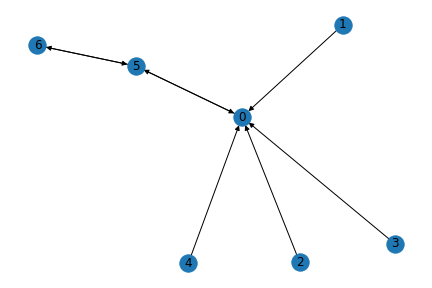
\includegraphics[width=0.55\linewidth]{directed_graph_example_unranked.png}
  \caption{This is an example of a weakly connected graph. If we start walking
  from $0$, $5$ or $6$ we can never reach vertices $1-4$. It is also not immediately
  clear which vertex $0$ or $5$ is more 'important'. While $0$ is directly
  connected to more vertices, $5$ may get more 'flow' through it since every
  path of length $2$ or more passes though it.}
  \label{fig:weaklyconnected}
\end{figure}

\begin{figure}[!htb]
  \centering
    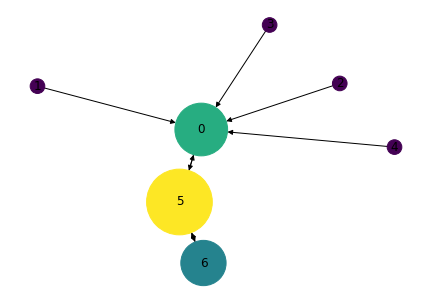
\includegraphics[width=0.55\linewidth]{directed_graph_example.png}
  \caption{The same graph with vertex size and color indicating its PageRank
  with parameter $\alpha=0.15$. We see that $5$ is ranked first, followed by
  $0$. The smaller the restart parameter, the more important $5$ will get
  because we allow for longer paths with fewer restarts.}
  \label{fig:weaklyconnectedpagedranked}
\end{figure}

\begin{figure}[!htb]
  \centering
    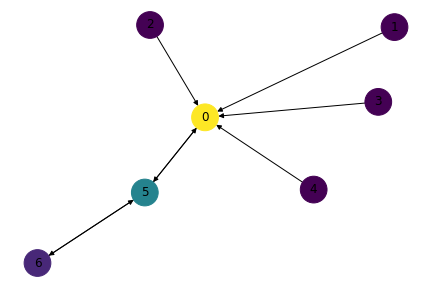
\includegraphics[width=0.55\linewidth]{directed_graph_example_tinyalpha.png}
  \caption{When the restart parameter is too large, the rank becomes almost
  uniform because the convex combination of the original graph with the
  $n$-clique graph of the restarts is weighted too heavily on the latter}
  \label{fig:weaklyconnectedpagedrankedbadly}
\end{figure}

\begin{figure}[!htb]
  \centering
    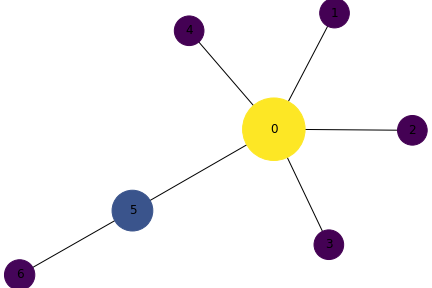
\includegraphics[width=0.55\linewidth]{undirected_graph_example.png}
  \caption{When we treat the graph as undirected and calculate the PageRanks
  ($\alpha=0.15$),
  Vertex $0$ comes this time on top. It is more central than $5$ and
  more random paths intersect it than any other vertex.}
  \label{fig:undirectedanked}
\end{figure}




\section{The Propagation Method}
The normalize adjacency matrix of 
a connected graph (for simplicity we use here undirected) is a transition matrix
and represents a
Markov process. On a given time-step, a visitor on a graph node chooses
his next station at random among the neighbours of the current station (node).

We want to know first, if we repeat this process to infinity will the frequency
of the visits at each node stabalize 

\section{testing}

\subsection{citations}

For more info see (textcite) \textcite[631]{meyer2000matrix}.

This is a normal (cite)~\cite[p.~115]{big}.

This is an (autocite) see \autocite[231]{lion2010}.

Change autocite in the usepackage definition to suit your needs. Use textcite if
you want to insert inline cite that includes the author's name.

Here is a~\cite{WikipediaPerronFrobenius} cite from wikipedia.

Just cite is just the normal citation command and nocite will make sure that the
reference appears in the bibliography even though it may have not specifically
been mentioned in the text somewhere.

\subsection{Images}

Here is an image

%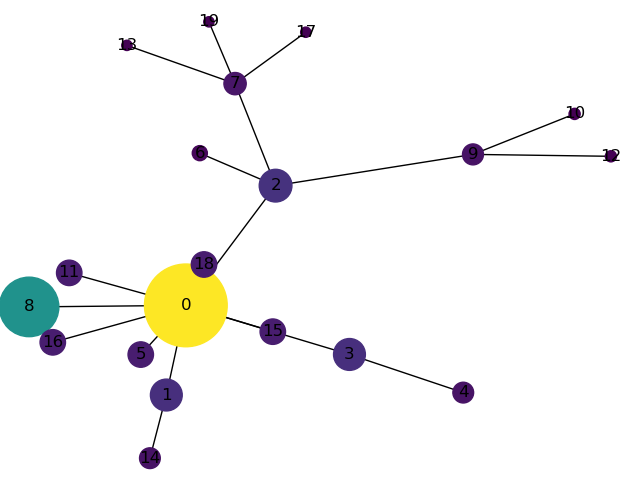
\includegraphics{BA20-1.png}

\begin{figure}[!htb]
  \centering
    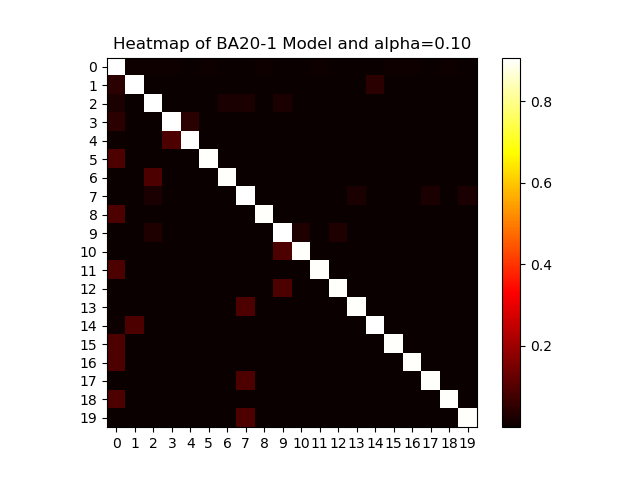
\includegraphics[width=0.65\linewidth]{Heatmap BA20-1 alpha=0.10.png}
  \caption{Heatmap. Alpha=0.1}
  \label{fig:heatmap}
\end{figure}

Refer to it with fig \ref{fig:heatmap} tada.


\begin{figure}[!htb]
  \centering
    
\includegraphics[width=0.65\linewidth]{test2.png}
  \caption{The apparatus used in the experiment. The forward right
  wing is fixed to the chain wheel which controls its elevation.
  The electrodes sticking out of the black precision clamp 
  are positioned to touch the exposed meso N1 at the root of the
  wing}
  \label{fig:apparatus}
\end{figure}

\subsection{Tables}

\begin{table}[!htb]
  \caption{Nernstsche Gleichgewichtspotenziale und das resultierende
  Membranpotenzial nach Goldmann Gleichung} 
\begin{center}
  \begin{tabular}{ | l | c | c | c | c | }
    \hline
     Ion & rel' Permeabilität &  Konz. in & Konz. auß & GG
     Potenzial \\ \hline
     $K^+$ & 1 & 124 & 4 & -86.74 \\
     $Na^+$ & 0.04 & 50 & 470 & 56.6 \\
     $Cl^-$ & 0.3 & 55 & 580 & -59.51 \\
    \hline
    $V_m$ &
    \multicolumn{4}{ | c |}{-51.35} \\
    \hline
  \end{tabular}
  \label{table:amp/dauer}
\end{center}
\end{table}

\section{Reference}
\printbibliography

\end{document}
